\section{Anforderungen}
Wie eingangs bereits beschrieben sollen lediglich die beiden Anwendungen "`Admin"' und "`VoteApp"' realisiert werden. In den folgenden Abschnitten werden die Anforderungen an die beiden Apps, sowie Entwürfe der Benutzeroberflächen vorgestellt. Eine gemeinsame Anforderung ist dabei die Lokalisierung in deutscher und englischer Sprache.

\subsection{Admin}
Das folgende Anwendungsfalldiagramm stellt die Anforderungen an den Admin dar:

\begin{figure}[H]
\centering
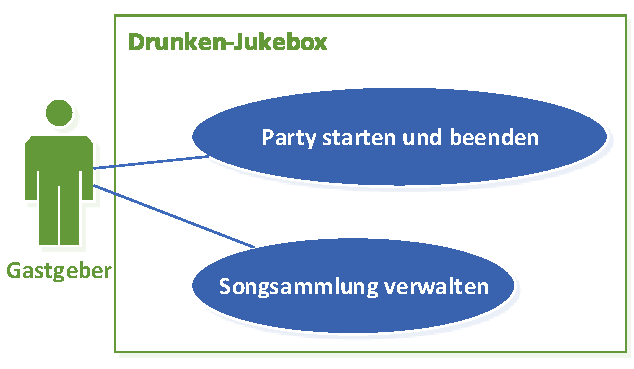
\includegraphics[width=0.7\linewidth]{Bilder/AdminUseCase}
\caption{Anwendungsfalldiagramm für den Admin}
\label{fig:AdminUseCase}
\end{figure}



Wir haben uns dazu entschieden eine eigene Oberfläche für den 



- Verwaltung von
  - Songs
  - Party
  
\begin{figure}[H]
\centering
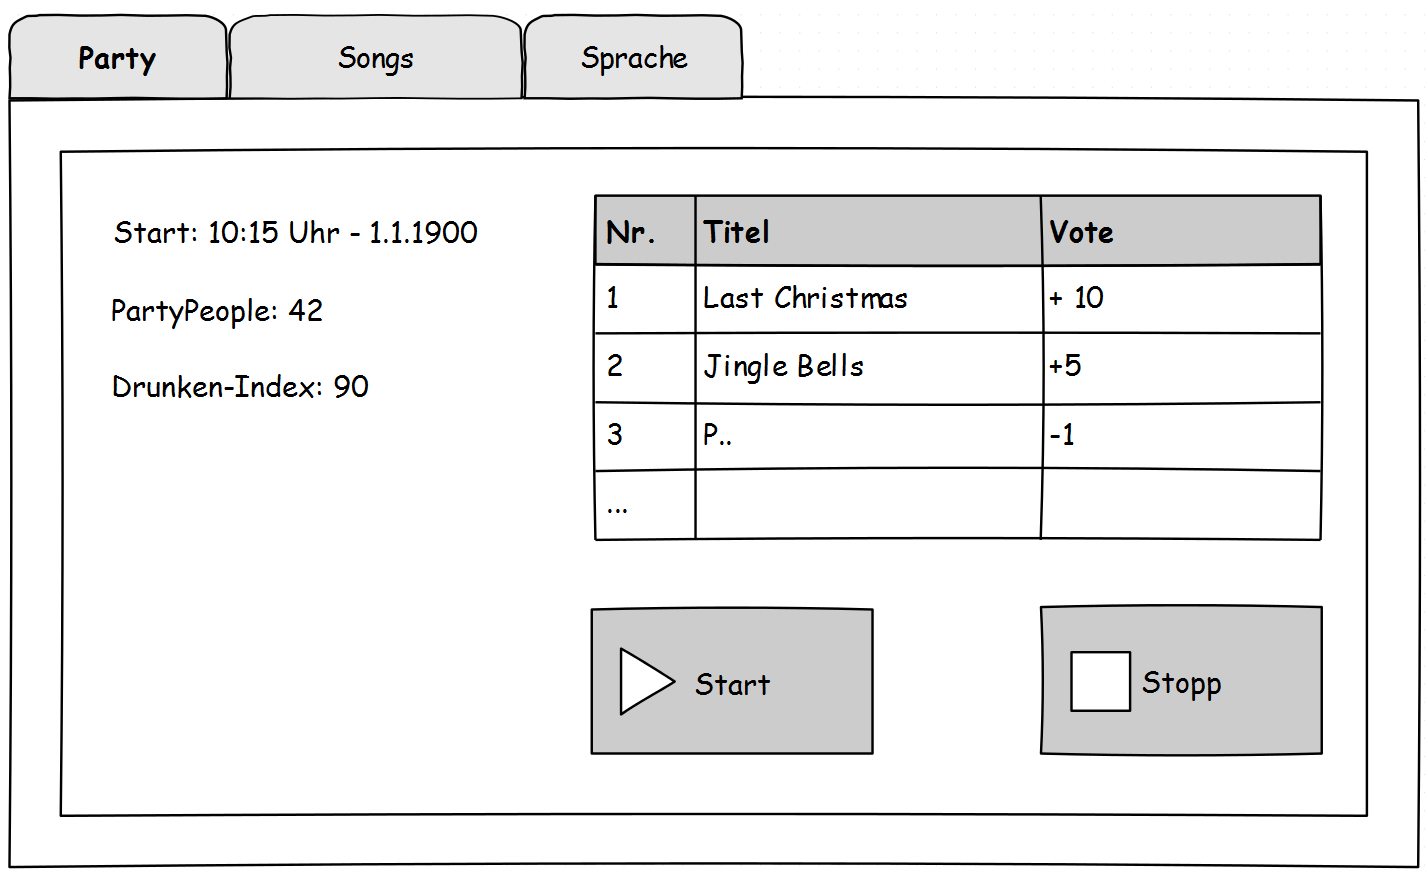
\includegraphics[width=0.95\linewidth]{Bilder/MockParty}
\caption{}
\label{fig:MockParty}
\end{figure}

\begin{figure}[H]
\centering
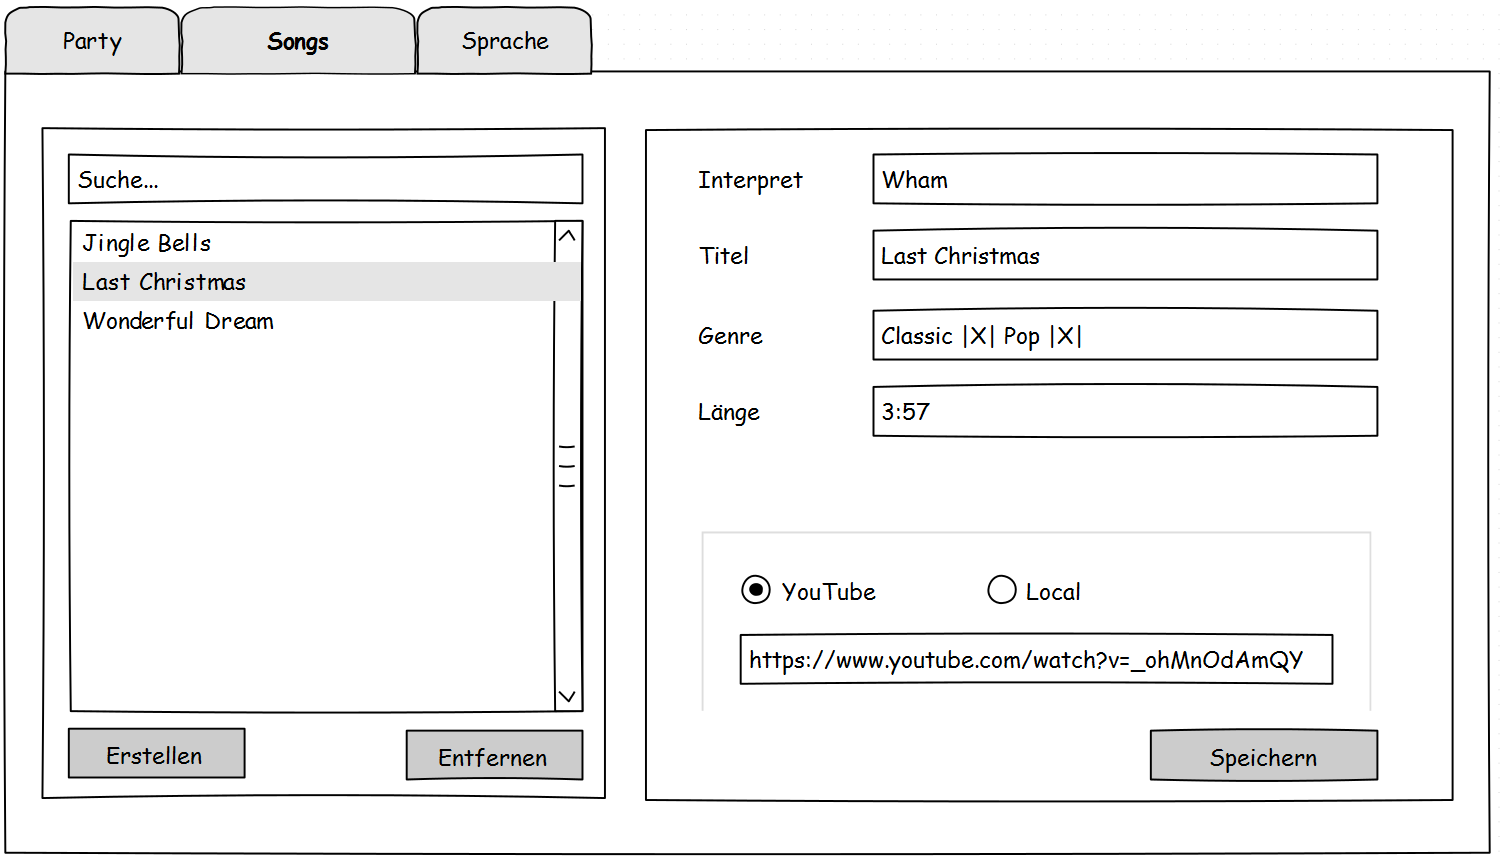
\includegraphics[width=0.95\linewidth]{Bilder/MockSongVerwaltung}
\caption{}
\label{fig:MockSongVerwaltung}
\end{figure}

  
Mockups einfügen und Funktionen erklären

\subsection{Vote-App}
- Anzeige der aktuellen Playlist (Send DI fehlt im Mockup)
- Voten
- DI (Mockup fehlt)

\begin{figure}[H]
\centering
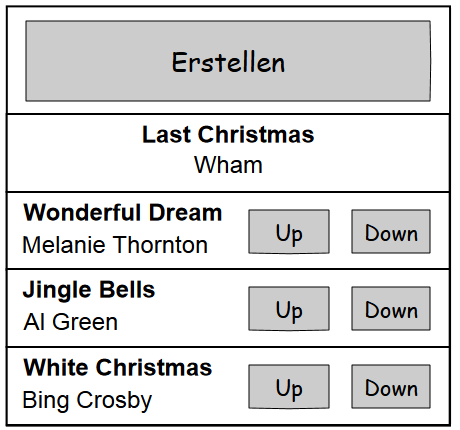
\includegraphics[width=0.6\linewidth]{Bilder/MockPartyPeopleClient}
\caption{}
\label{fig:MockPartyPeopleClient}
\end{figure}

\begin{figure}[H]
\centering
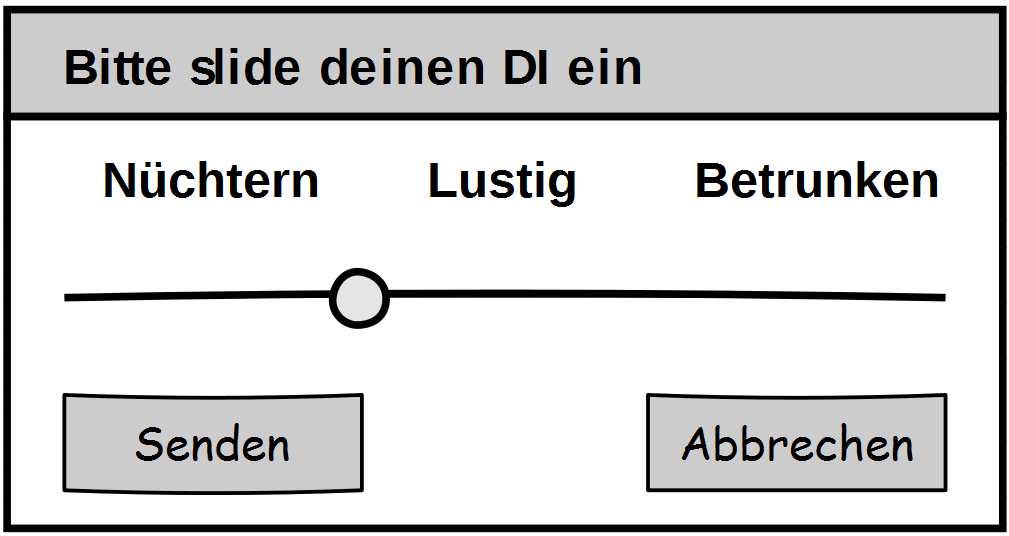
\includegraphics[width=0.7\linewidth]{Bilder/MockDiSlider}
\caption{}
\label{fig:MockDiSlider}
\end{figure}



Mockups einfügen und Funktionen erklären

Chris